\begin{figure}[htbp]
\section*{ TGFB3}
\centering
\begin{subfigure}[b]{0.95\textwidth}
\centering
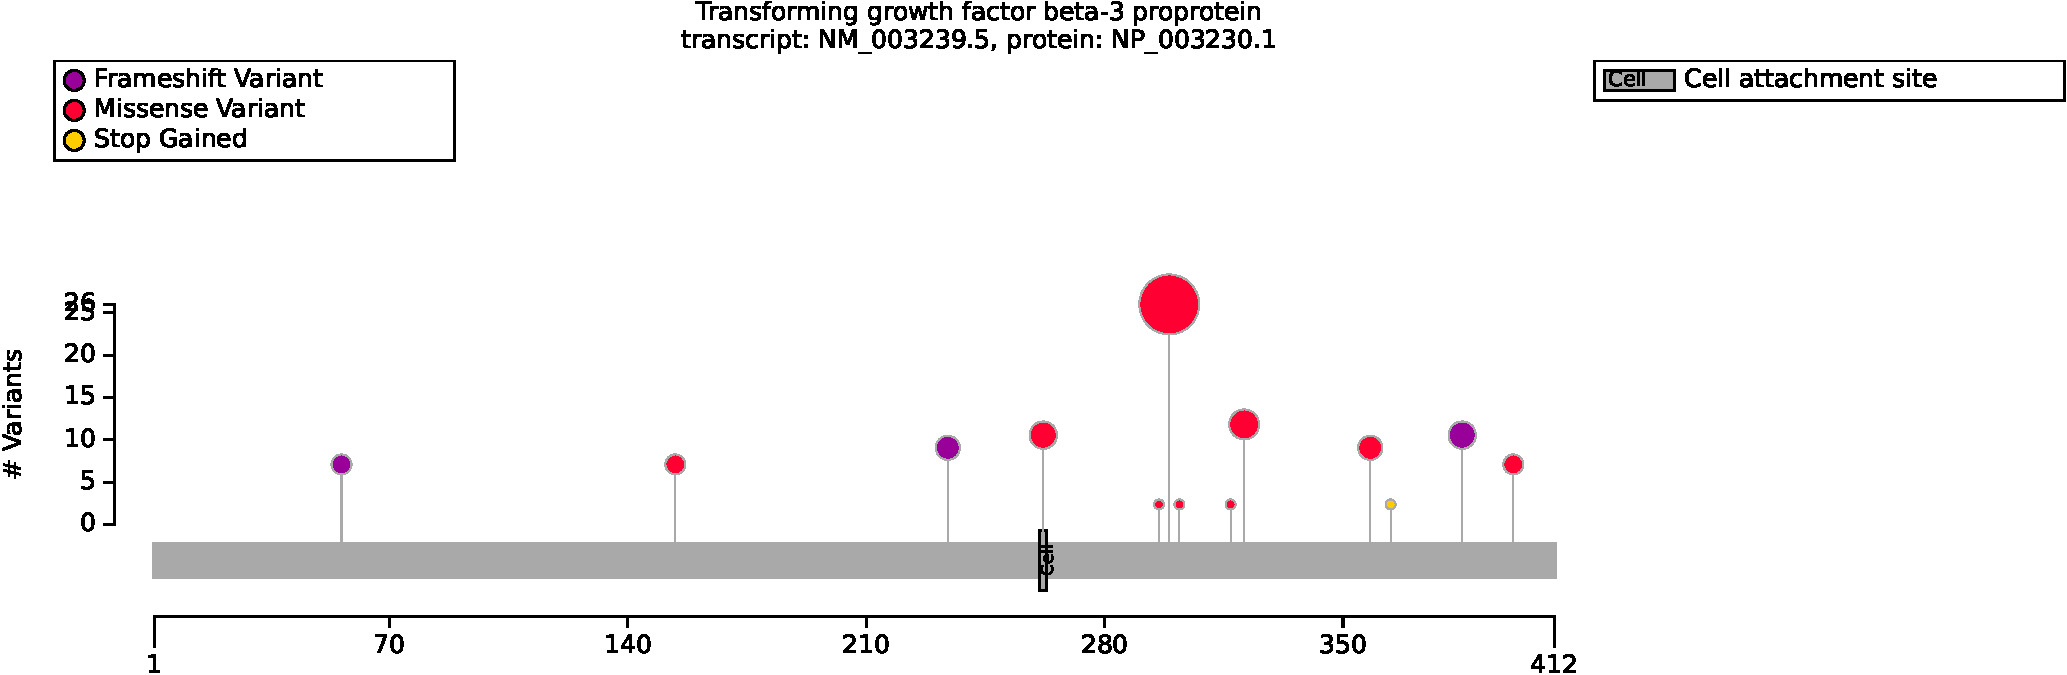
\includegraphics[width=\textwidth]{ img/TGFB3_protein_diagram.pdf} 
\captionsetup{justification=raggedright,singlelinecheck=false}
\caption{Distribution of variants in TGFB3}
\end{subfigure}

\vspace{2em}

\begin{subfigure}[b]{0.95\textwidth}
\centering
\resizebox{\textwidth}{!}{
\begin{tabular}{llllrr}
\toprule
Genotype (A) & Genotype (B) & total tests performed & significant results\\
\midrule
Missense & Other & 12 & 0\\
Asp263His & Other & 10 & 0\\
FEMALE & MALE & 13 & 0\\
\bottomrule
\end{tabular}
}
\captionsetup{justification=raggedright,singlelinecheck=false}
\caption{             Fisher Exact Test performed to compare HPO annotation frequency with respect to genotypes. }
\end{subfigure}

\vspace{2em}

\caption{ The cohort comprised 75 individuals (34 females, 41 males). 7 of these individuals were reported to be deceased. A total of 73 HPO terms were used to annotate the cohort. Disease diagnosis: Loeys-Dietz syndrome 5 (OMIM:615582). No significant correlations identified. A total of 75 unique variant alleles were found in \textit{TGFB3} (transcript: \texttt{NM\_003239.5}, protein id: \texttt{NP\_003230.1}).}
\end{figure}
